% !TEX root = pocs-2-project-revtex4.tex

%% replace 'startrek_dimensions' with short distinct tag
%% - helps with distinction for inclusion in other documents
%% - always

%% procedure for figures:
%% adding directory figures/localized/
%% before figures in includegraphics
%% commands forces search and localize

\section{Introduction}
\label{sec:startrek_dimensions.introduction}

\begin{figure}[tp!]
  \centering
    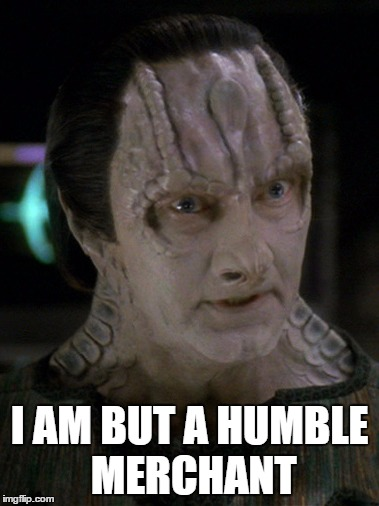
\includegraphics[width=0.5\columnwidth]{figures/localized/Garak.jpg}
  \caption{
    Garak, tailor and retired (?) spymaster.
  }
  \label{fig:startrek_dimensions.}
\end{figure}

\section{Description of data sets}
\label{sec:startrek_dimensions.data}

Transcripts of all episodes of \textit{Star Trek: The Original Series} (TOS), \textit{The Next Generation} (TNG) and \textit{Deep Space Nine} (DS9), as obtained from \href{http://chakoteya.net/StarTrek/index.html}{chakoteya.net} in February 2023. These are the first three live-action series of the Star Trek franchise. Further information about the corpus can be found in table \ref{table:series-comparison}.

\begin{table}
  \centering
  \renewcommand*{\arraystretch}{1.4}
  \rowcolors{2}{gray!15}{white}
  \begin{tabular}{l|c|c|c}
    \textbf{Series} & \textbf{Original Run} & \textbf{Episodes} & \textbf{Tokens / Episode} \\
    \hline
    \textbf{TOS} & 1966--1969 & 79 & 5603.51 \\
    \textbf{TNG} & 1987--1994 & 178 & 5389.92 \\
    \textbf{DS9} & 1993--1999 & 176 & 5756.46 \\
  \end{tabular}
  \caption{Comparison of corpi for Star Trek series: TOS, TNG, and DS9}
  \label{table:series-comparison}
\end{table}

\begin{figure}
  \centering
  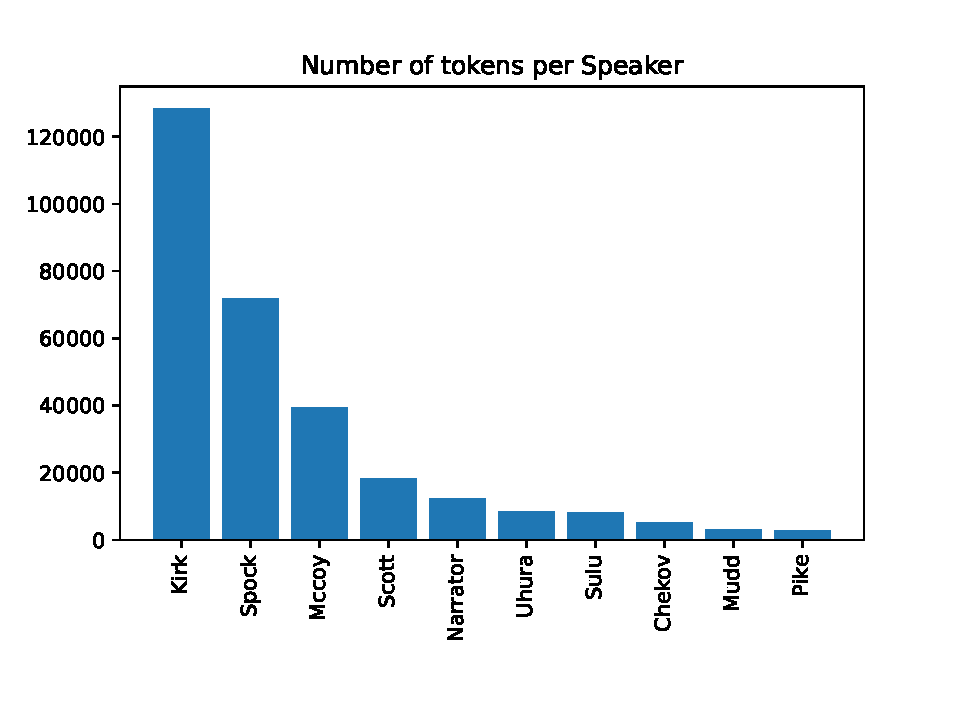
\includegraphics[width=\columnwidth]{figures/localized/tos_speaker_tokens.pdf}
  \caption{Number of words per speaker for the 10 most prolific speakers in \textit{Star Trek: The Original Series}.}
  \label{fig:tos_speaker_tokens}
\end{figure}

\begin{figure}
  \centering
  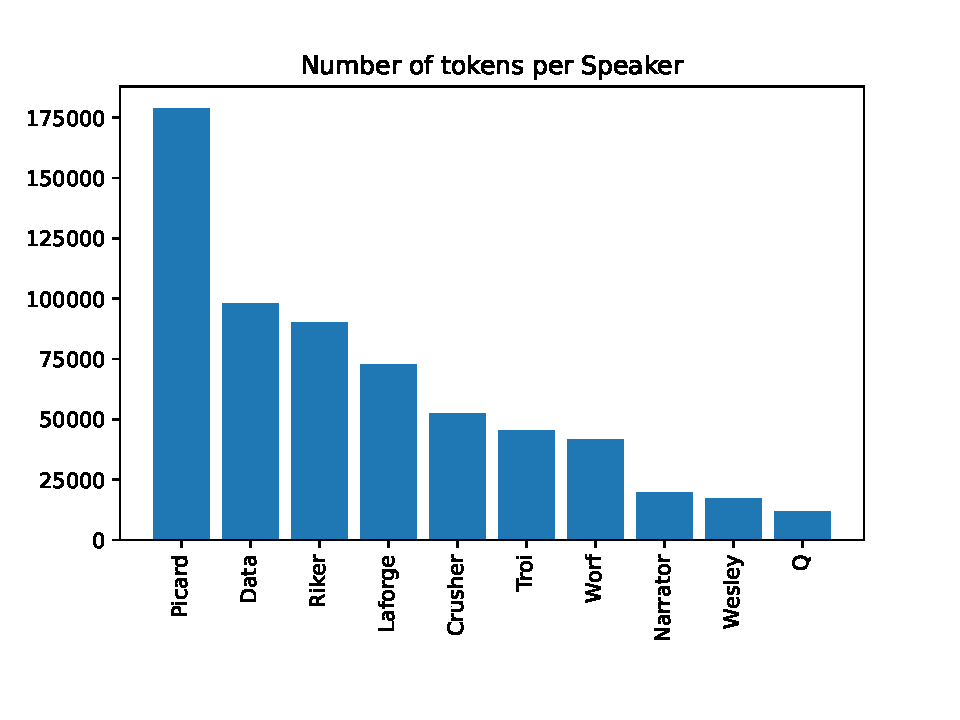
\includegraphics[width=\columnwidth]{figures/localized/tng_speaker_tokens.pdf}
  \caption{Number of words per speaker for the 10 most prolific speakers in \textit{Star Trek: The Next Generation}.}
  \label{fig:tng_speaker_tokens}
\end{figure}

\begin{figure}
  \centering
  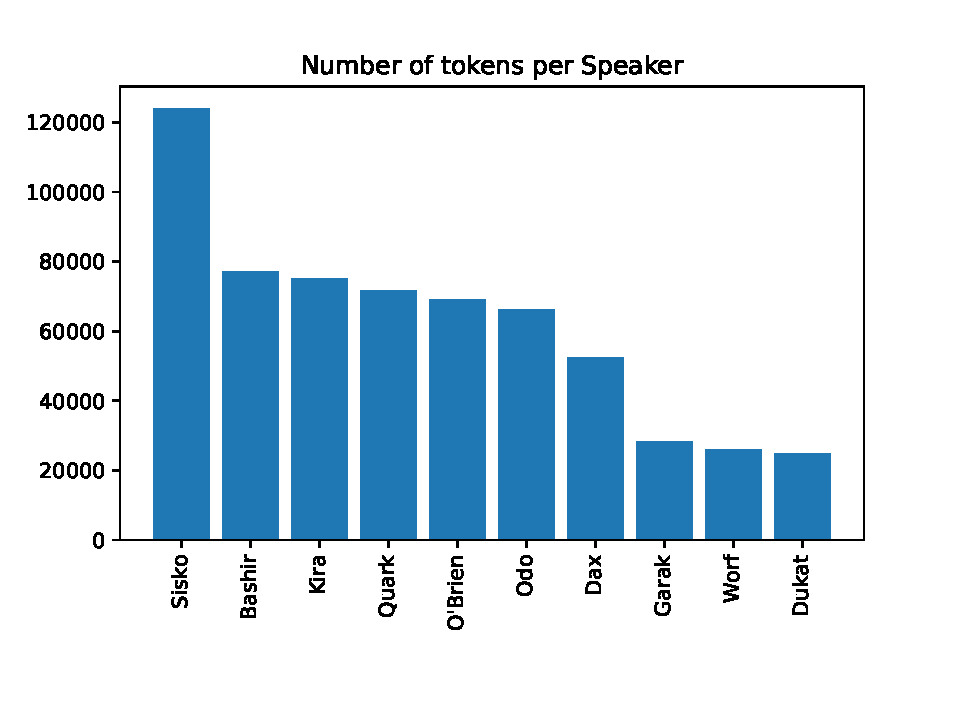
\includegraphics[width=\columnwidth]{figures/localized/ds9_speaker_tokens.pdf}
  \caption{Number of words per speaker for the 10 most prolific speakers in \textit{Star Trek: Deep Space Nine}.}
  \label{fig:ds9_speaker_tokens}
\end{figure}

Clearly visible in \ref{fig:tos_speaker_tokens}, \ref{fig:tng_speaker_tokens} and \ref{fig:ds9_speaker_tokens}: The respective Captain sticks out as the main character. But while TOS follows what looks like a power-law distribution, TNG has a stronger notion of a core cast, and DS9 even more so.

CAVEATS

Because the data sets do not contain timing information, we measure time in "words elapsed" as an approximation of real time.

The data set doesn't distinguish between the authors of log entries. Log entries are a commonly used instrument in Star Trek to convey information to the audience. They usually contain star date. All of these utterances are attributed to the special character called "Narrator". So for characters that author log entries (most entries are authored by the captain), we'll miss some of their speech when grouping by speaker.

\begin{figure}
  \centering
  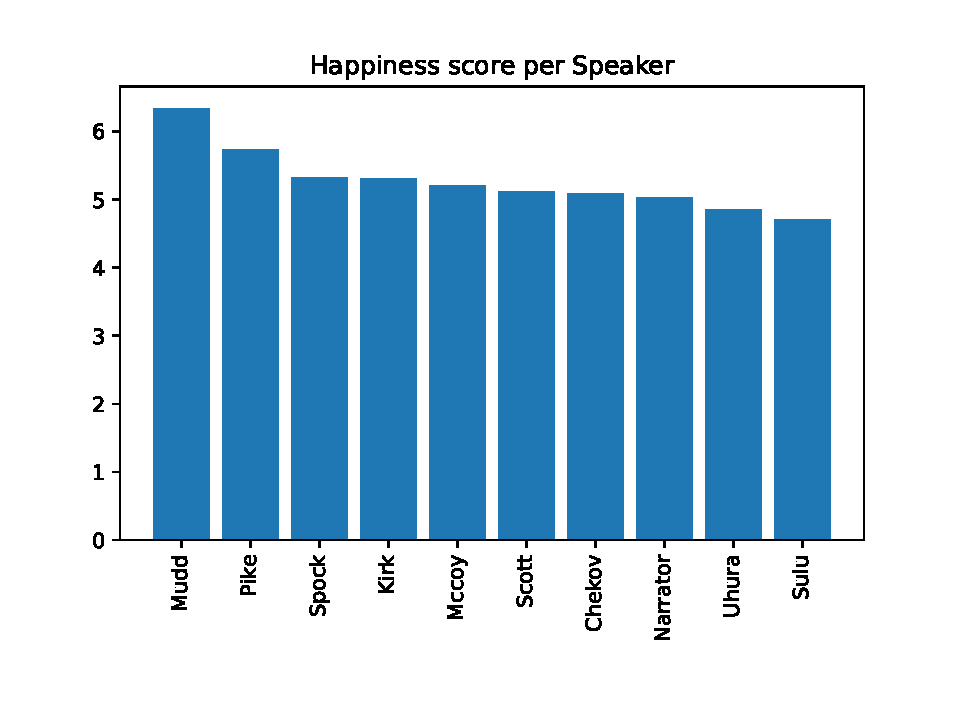
\includegraphics[width=\columnwidth]{figures/localized/tos_speaker_happiness_scores.pdf}
  \caption{Happiness score comparison of the 10 most prolific speakers in \textit{Star Trek: The Original Series}. Lens $[3, 7]$.}
  \label{fig:tos_happiness}
\end{figure}

\begin{figure}
  \centering
  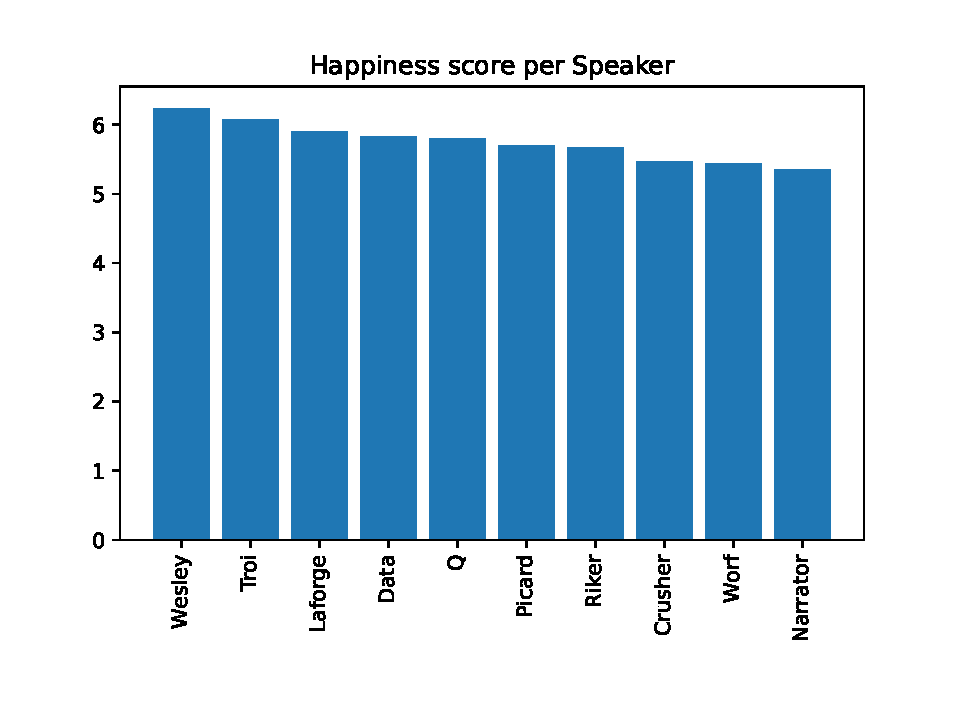
\includegraphics[width=\columnwidth]{figures/localized/tng_speaker_happiness_scores.pdf}
  \caption{Happiness score comparison of the 10 most prolific speakers in \textit{Star Trek: The Next Generation}. Lens $[3, 7]$.}
  \label{fig:tng_happiness}
\end{figure}

\begin{figure}
  \centering
  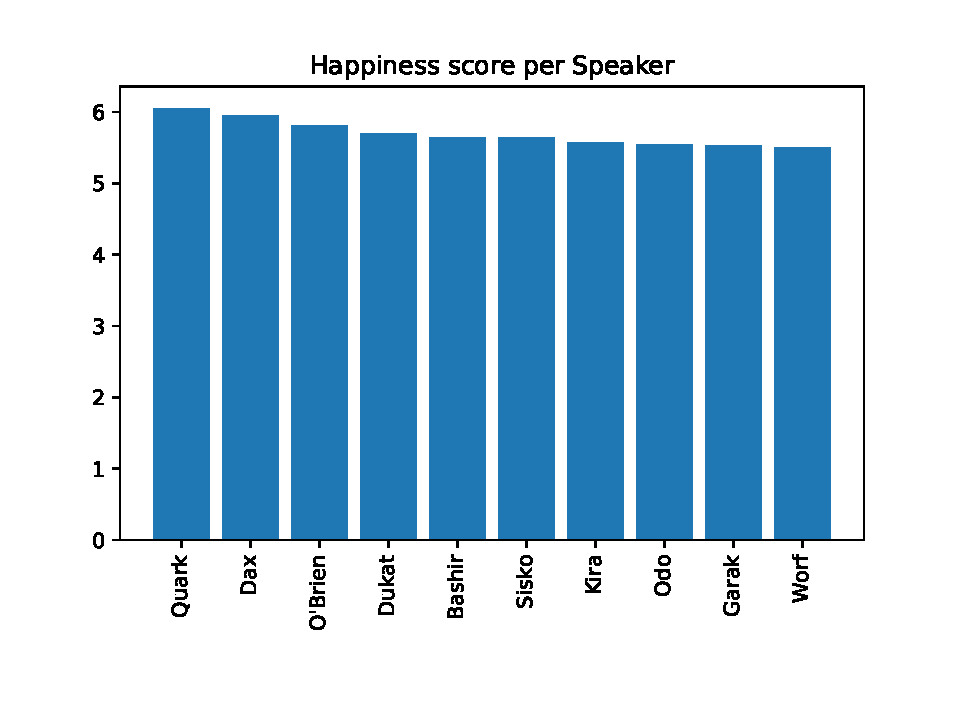
\includegraphics[width=\columnwidth]{figures/localized/ds9_speaker_happiness_scores.pdf}
  \caption{Happiness score comparison of the 10 most prolific speakers in \textit{Star Trek: Deep Space Nine}. Lens $[3, 7]$.}
  \label{fig:ds9_happiness}
\end{figure}

\section{Model}
\label{sec:startrek_dimensions.model}

\section{Results}
\label{sec:startrek_dimensions.results}

\todo{Explain what we found}

\begin{figure}
    \centering
    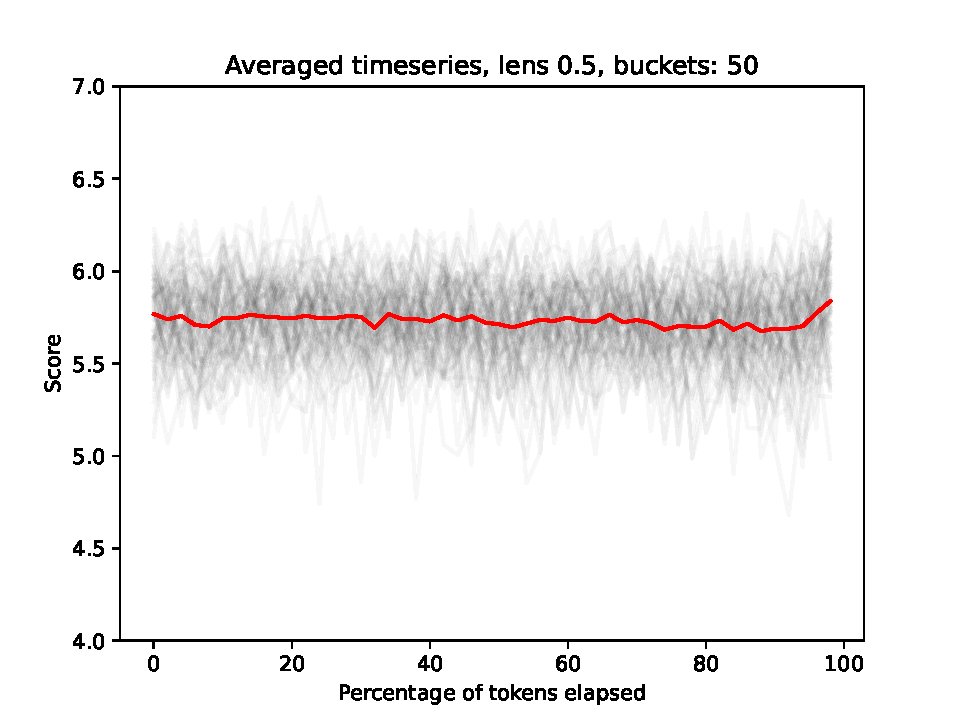
\includegraphics[width=\columnwidth]{figures/localized/average_episode_tos.pdf}
    \caption{Happiness timeseries of the average episode of Star Trek: The Original Series. Tokens are bucket so that we have the same number of data points for each episode. Episodes are plotted in black, the red line is the average.}
    \label{fig:average_episode_tos}
\end{figure}

\begin{figure}
    \centering
    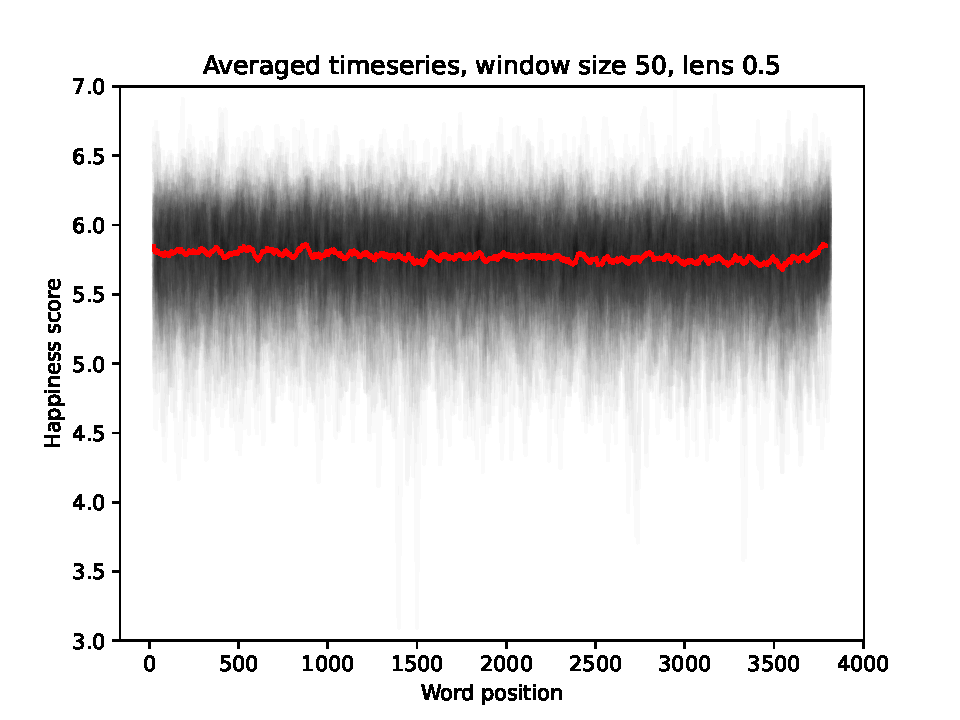
\includegraphics[width=\columnwidth]{figures/localized/average_episode_tng.pdf}
    \caption{Happiness timeseries of the average episode of Star Trek: The Next Generation. Episodes are scaled to the length of the shortest episode. Episodes are plotted in black, the red line is the average.}
    \label{fig:average_episode_tng}
\end{figure}

\begin{figure}
    \centering
    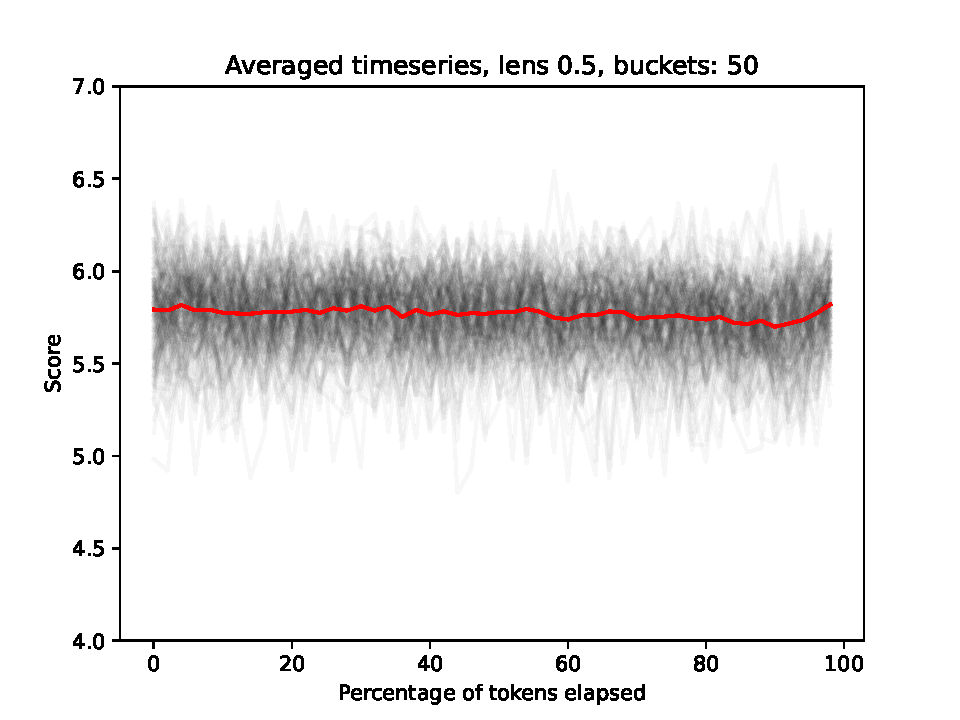
\includegraphics[width=\columnwidth]{figures/localized/average_episode_ds9.pdf}
    \caption{Happiness timeseries of the average episode of Star Trek: Deep Space Nine. Episodes are scaled to the length of the shortest episode. Episodes are plotted in black, the red line is the average.}
    \label{fig:average_episode_ds9}
\end{figure}

Visible in \ref{fig:average_episode_tos}, \ref{fig:average_episode_tng} and \ref{fig:average_episode_ds9}: The episodes usually have a happy end in all three series. Average happiness is comparable overall.

\section{Concluding remarks}
\label{sec:startrek_dimensions.concludingremarks}

\todo{Bring it home.}

\section{Future work}
\label{sec:startrek_dimensions.futurework}

\section{Methods}
\label{sec:startrek_dimensions.methods}

\todo{Add methods.}
